% Created 2021-06-09 Wed 11:19
% Intended LaTeX compiler: pdflatex
\documentclass[presentation, 8pt]{beamer}
\usepackage[utf8]{inputenc}
\usepackage[T1]{fontenc}
\usepackage{xcolor}
\usepackage{hyperref}
\usepackage{amsmath}
\usepackage{chessboard}
\ExplSyntaxOn %requires texlive 2020, in older system load expl3
\cs_new:Npn \getfieldnumber #1
{
\fp_eval:n { (\tl_tail:V #1 -1)*8 + \exp_args:Ne\int_from_alph:n{\tl_head:V #1} -1}
}
\ExplSyntaxOff

% features: (embed-files embed-tangled acronym underline par-sep image engraved-code-setup engraved-code)

  \usepackage[main,include]{embedall}
  \IfFileExists{./\jobname.org}{\embedfile[desc=The original file]{\jobname.org}}{}
  


\newcommand{\acr}[1]{\protect\textls*[110]{\scshape #1}}
\newcommand{\acrs}{\protect\scalebox{.91}[.84]{\hspace{0.15ex}s}}
\usepackage[normalem]{ulem}
\setlength{\parindent}{0pt}

\usepackage{graphicx}

  \usepackage{fvextra}
  \fvset{
    commandchars=\\\{\},
    highlightcolor=white!95!black!80!blue,
    breaklines=true,
    breaksymbol=\color{white!60!black}\tiny\ensuremath{\hookrightarrow}}
  \renewcommand\theFancyVerbLine{\footnotesize\color{black!40!white}\arabic{FancyVerbLine}}

  \definecolor{codebackground}{HTML}{f7f7f7}
  \definecolor{codeborder}{HTML}{f0f0f0}

  % TODO have code boxes keep line vertical alignment
  \usepackage[breakable,xparse]{tcolorbox}
  \DeclareTColorBox[]{Code}{o}%
  {colback=codebackground, colframe=codeborder,
    fontupper=\footnotesize,
    colupper=EFD,
    IfNoValueTF={#1}%
    {boxsep=2pt, arc=2.5pt, outer arc=2.5pt,
      boxrule=0.5pt, left=2pt}%
    {boxsep=2.5pt, arc=0pt, outer arc=0pt,
      boxrule=0pt, leftrule=1.5pt, left=0.5pt},
    right=2pt, top=1pt, bottom=0.5pt,
    breakable}
  
\definecolor{EFD}{HTML}{383a42}
\newcommand{\EFD}[1]{\textcolor{EFD}{#1}} % default
\definecolor{EFk}{HTML}{e45649}
\newcommand{\EFk}[1]{\textcolor{EFk}{#1}} % font-lock-keyword-face
\definecolor{EFd}{HTML}{84888b}
\newcommand{\EFd}[1]{\textcolor{EFd}{\textit{#1}}} % font-lock-doc-face
\definecolor{EFt}{HTML}{986801}
\newcommand{\EFt}[1]{\textcolor{EFt}{#1}} % font-lock-type-face
\definecolor{EFs}{HTML}{50a14f}
\newcommand{\EFs}[1]{\textcolor{EFs}{#1}} % font-lock-string-face
\definecolor{EFw}{HTML}{986801}
\newcommand{\EFw}[1]{\textcolor{EFw}{#1}} % font-lock-warning-face
\definecolor{EFb}{HTML}{a626a4}
\newcommand{\EFb}[1]{\textcolor{EFb}{#1}} % font-lock-builtin-face
\definecolor{EFct}{HTML}{9ca0a4}
\newcommand{\EFct}[1]{\textcolor{EFct}{#1}} % font-lock-comment-face
\definecolor{EFc}{HTML}{b751b6}
\newcommand{\EFc}[1]{\textcolor{EFc}{#1}} % font-lock-constant-face
\definecolor{EFpp}{HTML}{4078f2}
\newcommand{\EFpp}[1]{\textcolor{EFpp}{\textbf{#1}}} % font-lock-preprocessor-face
\definecolor{EFnc}{HTML}{4078f2}
\newcommand{\EFnc}[1]{\textcolor{EFnc}{\textbf{#1}}} % font-lock-negation-char-face
\definecolor{EFv}{HTML}{6a1868}
\newcommand{\EFv}[1]{\textcolor{EFv}{#1}} % font-lock-variable-name-face
\definecolor{EFf}{HTML}{a626a4}
\newcommand{\EFf}[1]{\textcolor{EFf}{#1}} % font-lock-function-name-face
\definecolor{EFcd}{HTML}{9ca0a4}
\newcommand{\EFcd}[1]{\textcolor{EFcd}{#1}} % font-lock-comment-delimiter-face
\definecolor{EFrc}{HTML}{4078f2}
\newcommand{\EFrc}[1]{\textcolor{EFrc}{\textbf{#1}}} % font-lock-regexp-grouping-construct
\definecolor{EFrb}{HTML}{4078f2}
\newcommand{\EFrb}[1]{\textcolor{EFrb}{\textbf{#1}}} % font-lock-regexp-grouping-backslash
\newcommand{\EFob}[1]{#1} % org-block
\definecolor{EFhn}{HTML}{da8548}
\newcommand{\EFhn}[1]{\textcolor{EFhn}{\textbf{#1}}} % highlight-numbers-number
\definecolor{EFhq}{HTML}{4078f2}
\newcommand{\EFhq}[1]{\textcolor{EFhq}{#1}} % highlight-quoted-quote
\definecolor{EFhs}{HTML}{986801}
\newcommand{\EFhs}[1]{\textcolor{EFhs}{#1}} % highlight-quoted-symbol
\definecolor{EFrdi}{HTML}{4078f2}
\newcommand{\EFrdi}[1]{\textcolor{EFrdi}{#1}} % rainbow-delimiters-depth-1-face
\definecolor{EFrdii}{HTML}{a626a4}
\newcommand{\EFrdii}[1]{\textcolor{EFrdii}{#1}} % rainbow-delimiters-depth-2-face
\definecolor{EFrdiii}{HTML}{50a14f}
\newcommand{\EFrdiii}[1]{\textcolor{EFrdiii}{#1}} % rainbow-delimiters-depth-3-face
\definecolor{EFrdiv}{HTML}{da8548}
\newcommand{\EFrdiv}[1]{\textcolor{EFrdiv}{#1}} % rainbow-delimiters-depth-4-face
\definecolor{EFrdv}{HTML}{b751b6}
\newcommand{\EFrdv}[1]{\textcolor{EFrdv}{#1}} % rainbow-delimiters-depth-5-face
\definecolor{EFrdvi}{HTML}{986801}
\newcommand{\EFrdvi}[1]{\textcolor{EFrdvi}{#1}} % rainbow-delimiters-depth-6-face
\definecolor{EFrdvii}{HTML}{4db5bd}
\newcommand{\EFrdvii}[1]{\textcolor{EFrdvii}{#1}} % rainbow-delimiters-depth-7-face
\definecolor{EFrdiix}{HTML}{80a880}
\newcommand{\EFrdiix}[1]{\textcolor{EFrdiix}{#1}} % rainbow-delimiters-depth-8-face
\definecolor{EFrdix}{HTML}{887070}
\newcommand{\EFrdix}[1]{\textcolor{EFrdix}{#1}} % rainbow-delimiters-depth-9-face
% end features
\usetheme{default}
\author{Jake Moss - s46409665}
\date{\today}
\title{Slides}
\hypersetup{
 pdfauthor={Jake Moss - s46409665},
 pdftitle={Slides},
 pdfkeywords={},
 pdfsubject={},
 pdfcreator={Emacs 28.0.50 (Org mode 9.5)}, 
 pdflang={English}}
\begin{document}

\maketitle
\section{Python implementation}
\label{sec:org59446c8}
\begin{frame}[label={sec:orgd7dac54},fragile]{Processing games}
 \begin{Code}
\begin{Verbatim}[]
\color[HTML]{383a42}\EFk{import} chess
\EFk{with} \EFb{open}(filename) \EFk{as} \EFv{pgn}:
    game = chess.pgn.read\_game(pgn) \EFcd{\# }\EFct{Parses pgn file}
    \EFv{board} = game.board()

    \EFk{for} move \EFk{in} game.mainline\_moves():
        board.push(move) \EFcd{\# }\EFct{Pushs the move to the move stack, this "makes" the move}
\end{Verbatim}
\end{Code}
\end{frame}
\section{Luxcore}
\label{sec:org4dd6641}
\begin{frame}[label={sec:org4da1645}]{Incompatibility}
\begin{center}
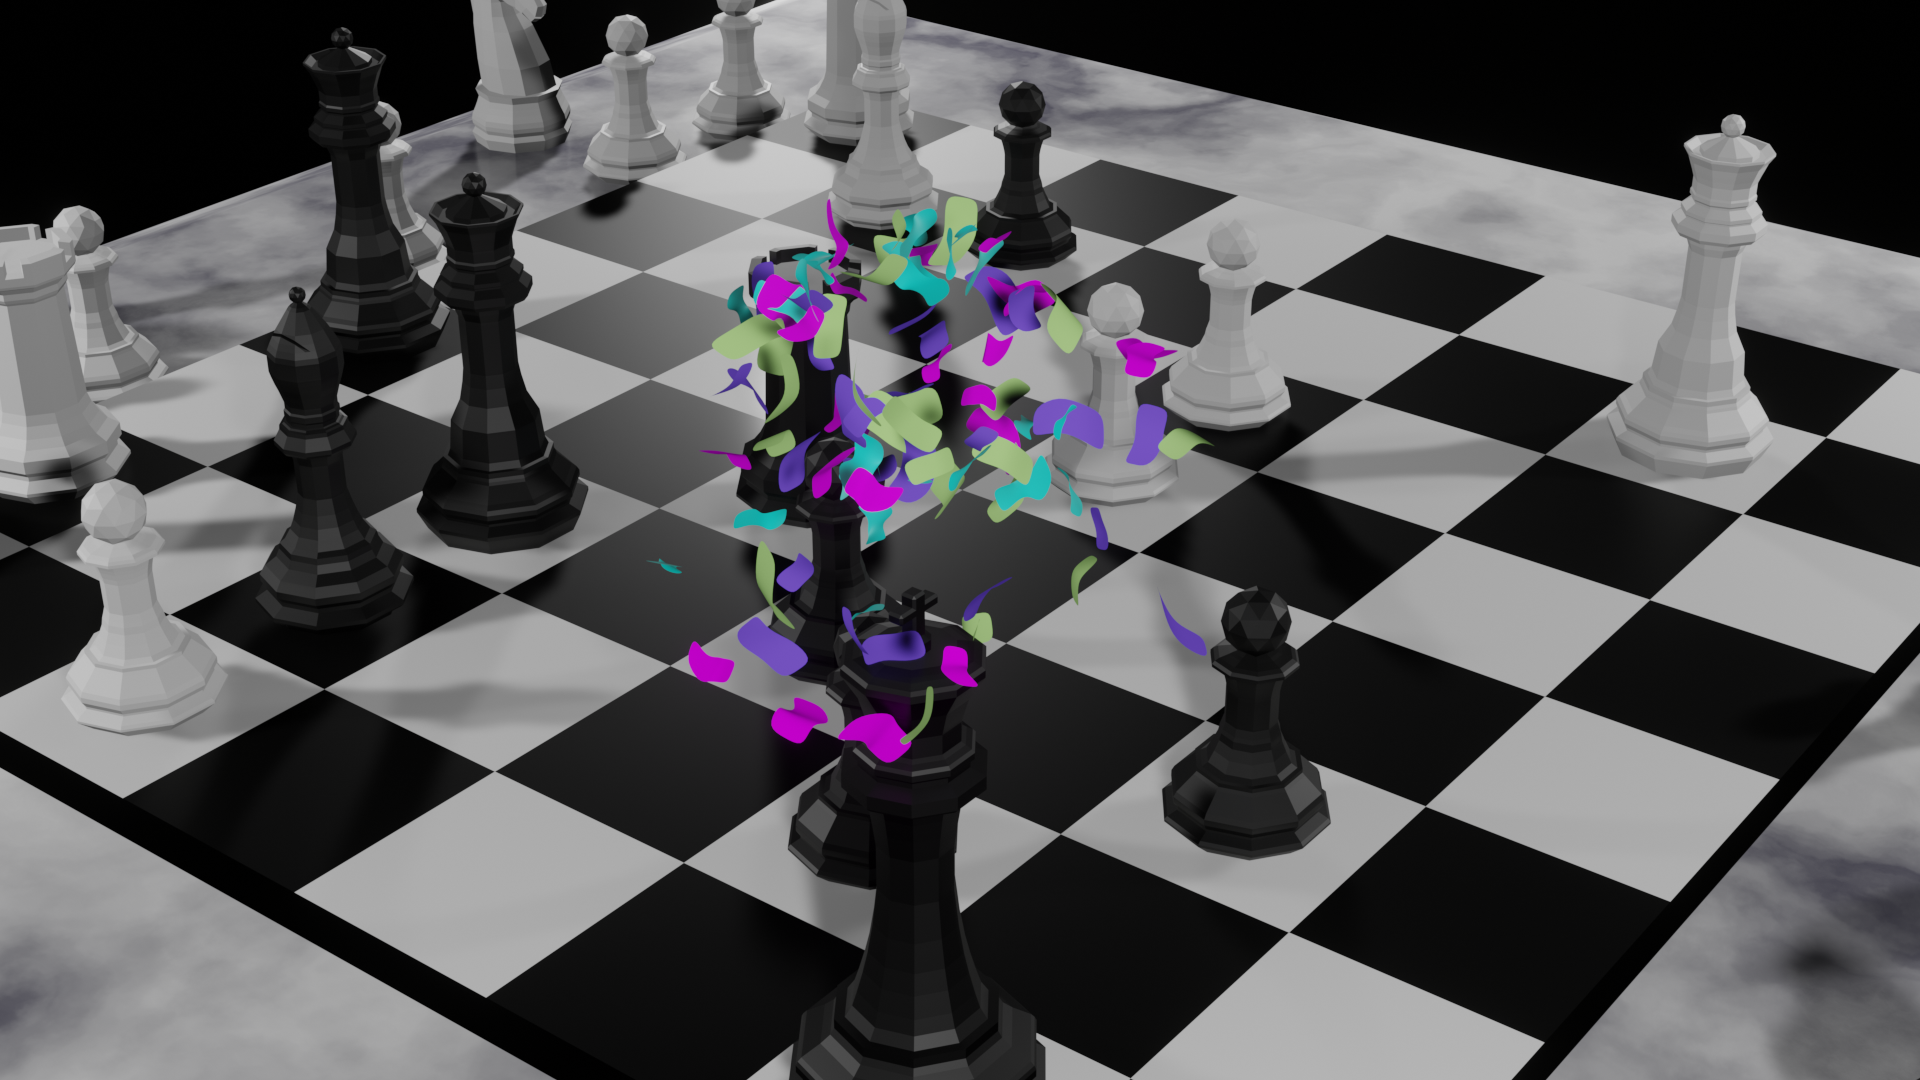
\includegraphics[width=.9\linewidth]{Images/luxcore fail-eevee.png}
\end{center}
\end{frame}
\begin{frame}[label={sec:orgd515b4a}]{Incompatibility}
\begin{center}
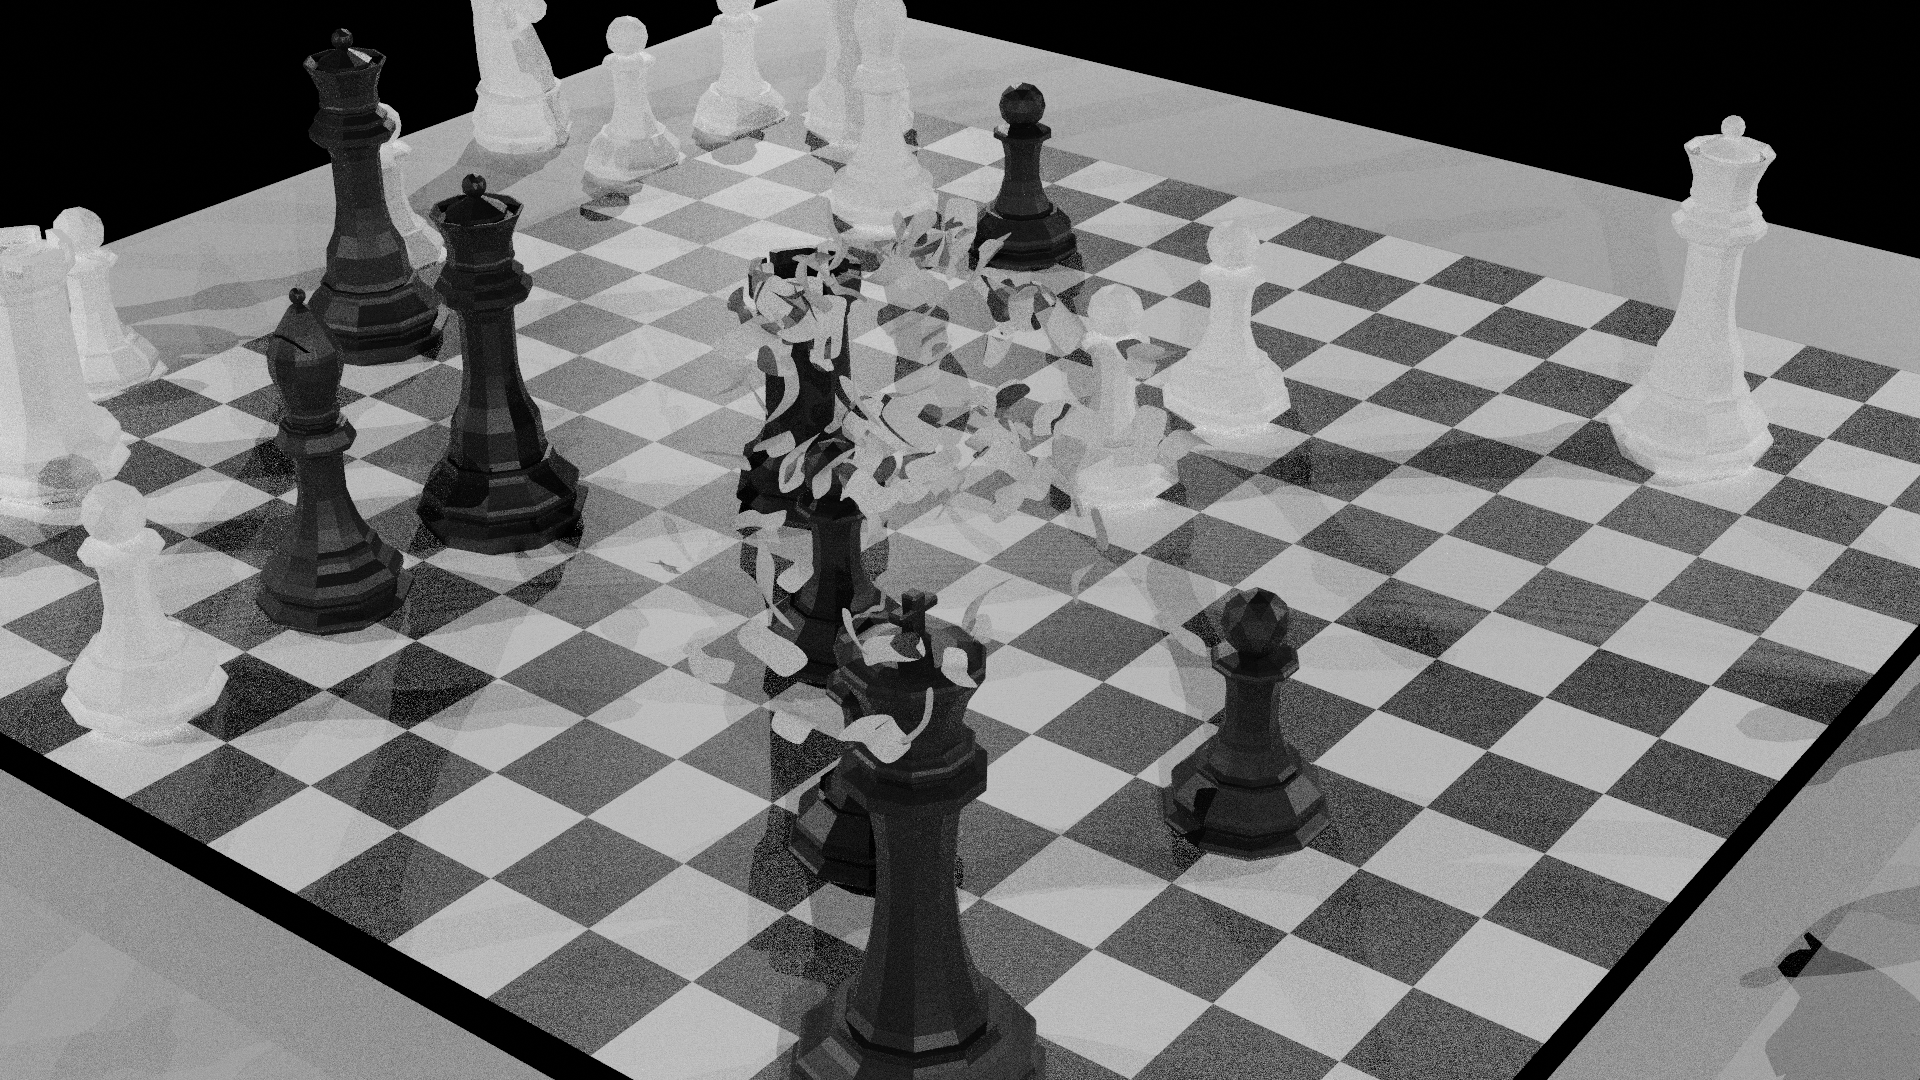
\includegraphics[width=.9\linewidth]{Images/luxcore fail.png}
\end{center}
\end{frame}
\begin{frame}[label={sec:org5813c26}]{Incompatibility}
\begin{itemize}
\item Confetti texture
\item Check board texture
\item Marble texture
\end{itemize}
\end{frame}
\begin{frame}[label={sec:org476e136}]{Checker texture fix}
\begin{columns}
\begin{column}{0.45\columnwidth}
\begin{block}{Eevee}
\begin{center}
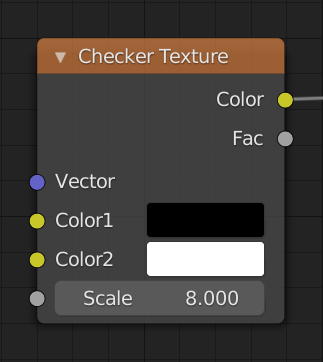
\includegraphics[width=.9\linewidth]{Images/checktexture-fix.png}
\end{center}
\end{block}
\end{column}
\begin{column}{0.45\columnwidth}
\begin{block}{Luxcore}
\begin{center}
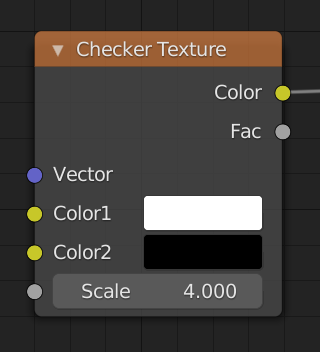
\includegraphics[width=.9\linewidth]{Images/checktexture-fix-luxcore.png}
\end{center}
\end{block}
\end{column}
\end{columns}
\end{frame}
\end{document}
